\section{Stabilità di sistemi LTI}
Quando un sistema è sottoposto a un ingresso, è importante capire se la
risposta del sistema rimarrà limitata o se divergerà nel tempo. La stabilità
previene che il sistema assuma valori distanti dalle condizioni iniziali,
garantendo che la risposta del sistema rimanga entro limiti accettabili. Per
sovrapposizione degli effetti, posso differenziare tra la risposta zero-input
(ZI) e la risposta zero-state (ZS). La risposta ZI è la risposta del sistema
quando l'ingresso è nullo, mentre la risposta ZS è la risposta del sistema
quando le condizioni iniziali sono nulle. Quando la risposta libera dello stato
la stabilità è interna, mentre quando la risposta forzata dell'uscita è
stabile, allora la stabilità è di tipo BIBO (Bounded-Input, Bounded-Output).
\subsection{Definizione formale di stabilità}
\begin{tcolorbox}[title=Sistema internamente stabile, colback=blue!5!white,colframe=blue!75!black]
    Un sistema LTI è detto internamente stabile se la risposta zero-input
    (risposta libera dello stato) rimane limitate per ogni possibile valore
    delle condizioni iniziali.
\end{tcolorbox}
\begin{tcolorbox}[title=Sistema asintoticamente stabile, colback=green!5!white,colframe=green!75!black]
    Un sistema è asintoticamente stabile se la risposta libera dello stato
    converge a zero qualsiasi sia la condizione iniziale $x_0$.

\end{tcolorbox}
\begin{tcolorbox}[title=Sistema instabile, colback=red!5!white,colframe=red!75!black]
    Un sistema si dice instabile se è esiste almeno una condizione iniziale
    $x_0$ per cui la risposta libera dello stato diverge.
\end{tcolorbox}

\subsection{Come si deduce se un sistema è internamente stabile?}
Per dedurre se un sistema è internamente stabile, è necessario analizzare la
sua risposta zero-input (ZI). Nel dominio del tempo, la risposta ZI è data da:
\begin{equation}
    x_{zi}(t) = e^{At} x(0)
\end{equation}
Per ulteriore semplicità, andiamo a calcolare la trasformata di Laplace della
risposta ZI, che è data da:
\begin{equation}
    X_{zi}(s) = (sI - A)^{-1} x(0)
\end{equation}
Sapendo che $(sI-A)^{-1}$ ottengo che:
\begin{equation}
    (sI - A)^{-1} = \frac{1}{\det(sI - A)} \text{Adj}(sI - A) = \frac{[a_{ij}]}{p_A(s)}
\end{equation}
dove $p_A(s) = \det(sI - A)$ è il polinomio caratteristico del sistema.
\newpage
Analizzando le radici del polinomio caratteristico, è possibile dedurre che:
\begin{itemize}
    \item Se tutte le radici del polinomio caratteristico hanno \textbf{parte reale
              negativa} e \textbf{molteplicità 1}, allora il sistema è
          \textbf{asintoticamente stabile}.
    \item Se almeno una radice del polinomio caratteristico ha \textbf{parte reale
              positiva} e \textbf{molteplicità 1}, allora il sistema è \textbf{instabile}.
    \item Se almeno una radice del polinomio caratteristico ha \textbf{parte reale
              nulla}, \textbf{molteplicità 1} e tutte le altre radici hanno parte reale
          negativa, allora il sistema è \textbf{marginalmente stabile}, quindi bounded.
\end{itemize}
Capire bene la parte della molteplicità delle radici

Se la molteplicità di una radice è maggiore di 1, distinguiamo tra i seguenti
casi:
\begin{itemize}
    \item \textbf{Interna stabilità}: se e solo se tutte le radici del polinomio
          caratteristico hanno parte reale negativa, indipendentemente dalla
          molteplicità.
    \item \textbf{Instabilità}: se esiste almeno una radice del polinomio
          caratteristico (autovalore) con parte reale positiva,
          indipendentemente dalla molteplicità. Oppure tutti gli autovalori
          hanno parte reale negativa, ma esiste almeno una radice con
          molteplicità maggiore di 1.
\end{itemize}
\subsection{Stabilità BIBO: stabilità esterna}
Un sistema BIBO studia quando un sistema è stabile in termini di ingresso e
uscita nei limiti di un certo intervallo.
\begin{equation}
    \forall u_M \epsilon (0, \infty), \exists y_M \epsilon (0, \infty) : |u(t)| < u_M, \forall t \geq 0 \Rightarrow |y(t)| < y_M, \forall t \geq 0
\end{equation}
\begin{tcolorbox}
    La BIBO stabilità è relativa al comportamento della risposta forzata
    dell'uscita. La risposta dell'uscita è:
    \begin{equation}
        y(t) = \mathbb{L}^{-1} \{Y(s)\}
    \end{equation}
    \begin{equation}
        Y(s) = C (sI - A)^{-1} x(0) + {[}C (sI - A)^{-1} B + D{]} U(s)
    \end{equation}
    Siccome stiamo considerando solo la risposta forzata dell'uscita, a noi
    interessa solo la parte $Y_{zs}(s) = {[}C (sI - A)^{-1} B + D{]} U(s)$, che
    è la matrice di trasferimento del sistema forzato. Per assunto sappiamo che:
    \begin{equation}
        Y(s) = H_{zs}(s) U(s) = \frac{N_H(s)}{D_H(s)} \frac{N_U(s)}{D_U(s)}
    \end{equation}
    Procediamo facendo la scomposizione in fratti semplici di $Y(s)$:
    \begin{multline}
        Y(s) = \frac{N_H(s)}{(s-p_1^{H})^{\alpha_1^H} \cdots (s-p_1^{U})^{\beta_1^U} \cdots} \\
        = \frac{R_{1,1}^H}{(s-p_1^{H})} + \frac{R_{1,2}^H}{(s-p_1^{H})^2} + \cdots + \frac{R_{1,1}^U}{(s-p_1^{U})} + \frac{R_{1,2}^U}{(s-p_1^{U})^2} + \cdots
    \end{multline}
    \begin{equation}
        y(t) = \mathbb{L}^{-1} \{Y(s)\} = R_{1,1}^H e^{p_1^{H}t} + \cdots
    \end{equation}
\end{tcolorbox}
\begin{tcolorbox}
    RECUPERA TUTTO
\end{tcolorbox}
\subsection{Stabilità di un equilibro di soluzione}
Chiamiamo punto di equilibrio stabile se tutte le soluzioni partono vicino a
$\bar{x}$ e rimane vicino per tutto il tempo. Invece, chiamiamo un punto
asintoticamente stabile se parte vicino a $\bar{x}$ e converge a $\bar{x}$ per
t che tende a infinito. Infine, chiamiamo un punto di equilibrio instabile se
esiste una soluzione che parte vicino a $\bar{x}$ ma si allontana da $\bar{x}$
per t che tende a infinito. Un punto di equilibrio è stabile definito da:
\begin{equation}
    \forall \epsilon > 0, \exists \delta > 0 : ||x(0) - \bar{x}|| \leq \delta \Rightarrow ||x(t) - \bar{x}|| \leq \epsilon, \forall t \geq 0
\end{equation}
Se vogliamo definire un punto di equilibrio asintoticamente stabile, abbiamo
che:
\begin{equation}
    \lim_{t \to \infty} ||x(t) - \bar{x}|| = 0
\end{equation}
\begin{figure}[h!]
    \centering
    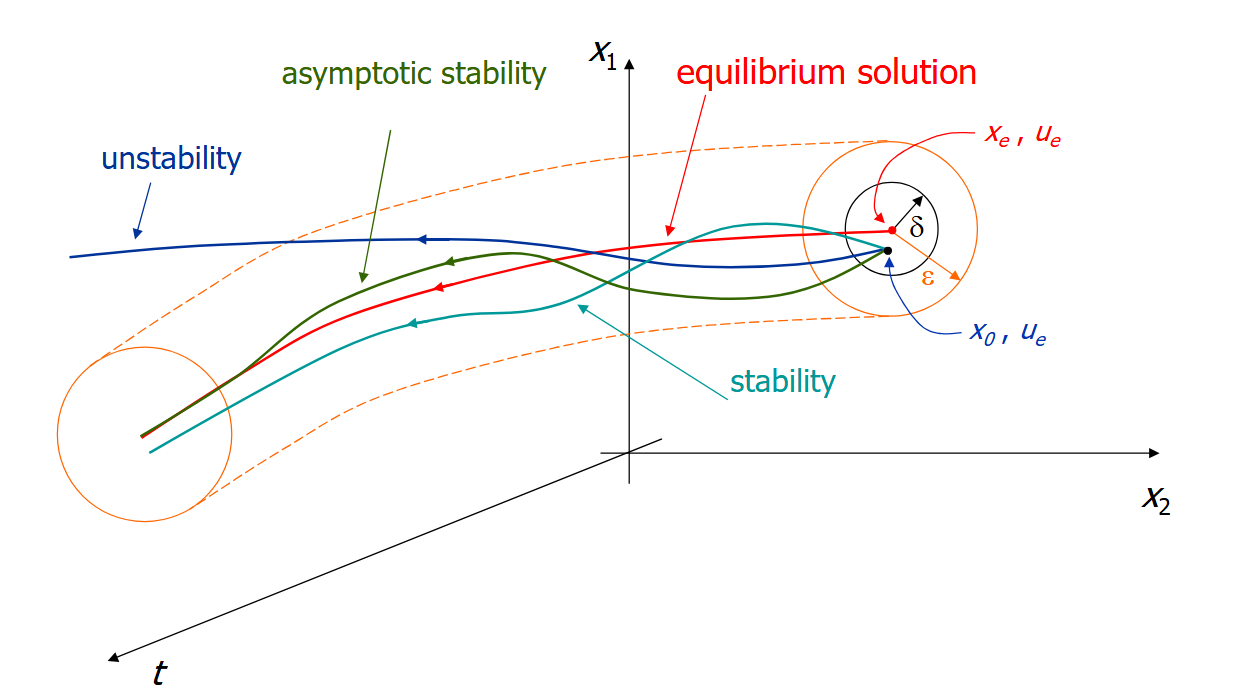
\includegraphics[width=0.5\textwidth]{foto/cph4/equilibrio.png}
    \caption{Equilibrio}
\end{figure}

\begin{minipage}{0.6\textwidth}
    Lo studioso russo Lyapunov ha dimostrato che se esiste una funzione $V(x)$,
    chiamata funzione di Lyapunov, che soddisfa le seguenti condizioni:
    \begin{itemize}
        \item $V(x)$ è definita positiva, ovvero $V(x) > 0$ per ogni $x \neq
                  \bar{x}$ e $V(\bar{x}) = 0$.
        \item La derivata di $V(x)$ lungo le traiettorie del sistema è definita negativa,
              ovvero $\dot{V}(x) < 0$ per ogni $x \neq \bar{x}$.
        \item $V(x)$ è radiale limitata, ovvero $V(x) \to \infty$ quando $||x||
                  \to \infty$.
    \end{itemize}
\end{minipage}
\hfill
\begin{minipage}{0.35\textwidth}
    
\includegraphics[width=0.75\textwidth]{foto/cph4/lyapunov.png}
\end{minipage}
\newline
\newline
\newline
Allora il punto di equilibrio $\bar{x}$ è asintoticamente stabile. In altre
parole, se esiste una funzione di Lyapunov che soddisfa queste condizioni,
allora tutte le soluzioni del sistema convergono a $\bar{x}$ quando $t$ tende a
infinito.
\subsection{Stabilità di un equilibrio di soluzione attraverso un modello lineare}
Supponiamo di avere un sistema non lineare descritto da:
\begin{equation}
    \dot{x}(t) = f(x(t), u(t))
\end{equation}
Assumiamo A pari a:
\begin{equation}
    A = \frac{\partial f(x)}{\partial x} \big{|}_{x = \bar{x}, u = \bar{u}}
\end{equation}
l'equilibrio è asintoricamente stabile se tutte le radici del polinomio
caratteristico di A hanno parte reale negativa, mentre è instabile se esiste
almeno una radice del polinomio caratteristico di A con parte reale positiva. Se
esiste almeno una radice del polinomio caratteristico di A con parte reale
nulla, allora il sistema è marginalmente stabile, quindi bounded.

Riassumendo: \newline \newline
\begin{minipage}{0.45\textwidth}
    \begin{center}
        \begin{tabular}{|c|c|c|}
            \hline
            \textbf{Parte reale} & \textbf{Molteplicità} & \textbf{Stabilità}    \\
            \hline
            Negativa             & Qualsiasi             & Asintoticamente
            stabile
            \\ \hline
            Positiva             & Qualsiasi             & Instabile             \\ \hline
            Nulla                & 1                     & Marginalmente stabile
            \\ \hline
            Nulla                & $>$ 1                 & Instabile             \\ \hline
        \end{tabular}
    \end{center}
\end{minipage}
\hfill
\begin{minipage}{0.45\textwidth}
    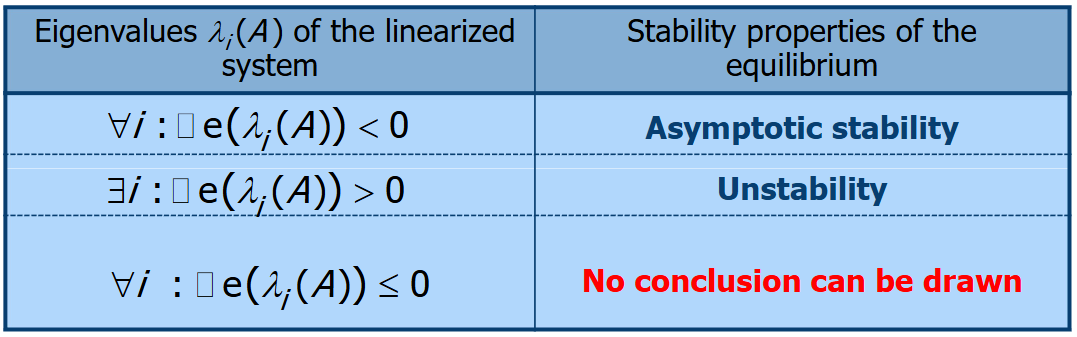
\includegraphics[width=\textwidth]{foto/cph4/stability.png}
\end{minipage}
Tendenzialmente cercheremo di studiare casi in cui il sistema è asintoticamente
stabile.
\subsection{Introduzione al controllo di un sistema dinamico LTI}
\begin{equation}
    S = \begin{cases}
        \dot{x}(t) = A x(t) + B u(t) \\
        y(t) = C x(t) + D u(t)
    \end{cases}
\end{equation}
\begin{itemize}
    \item Studiando il comportamento di un sistema dinamico LTI abbiamo definito e
          analizzato un'importante proprietà che abbiamo chiamato
          \textbf{\textit{Stabilità}};
    \item Abbiamo dedotto che la stabilità interna del sistema LTI dipende dagli
          autovalori di A;
    \item Abbiamo anche capito che quando progettiamo un sistema di controllo noi
          vogliamo ottenere alla fine del progetto un sistema asintoticamente stabile,
          perché:\begin{itemize}
              \item l'effetto delle condizioni iniziali $x(\phi)$ va a 0 per $t \to \infty$;
              \item sistama BIBO stabile, quando applico ingressi di ampiezze limitate, ottengo che
                    le $y(t)$ rimangono limitate;
          \end{itemize}
    \item Dall'analisi dei modi della risposta di un sistema LTI possiamo inoltre dedurre
          che le principali caratteristiche delle risposta (presenza/assenza di
          oscillazioni, velocità di risposta etc) dipendono da come sono fatti gli
          autovalori di A.
    \item Il mio obietivo potrebbe quindi essere quello di partire da un sistema da
          controllare:
          \begin{equation}
              S = \begin{cases}
                  \dot{x}(t) = A x(t) + B u(t) \\
                  y(t) = C x(t) + D u(t)
              \end{cases}
          \end{equation}
          con autovalori di A che non ci piacciono, allora noi vogliamo ottenere
          un nuovo sistema:
          \begin{equation}        S' = \begin{cases}
                  \dot{x}(t) = A' x + ... \\
                  y(t) = C' x + ...
              \end{cases}
          \end{equation}
          in cui gli autovalori di $A'$ sono quello che ci piacciono. Per fare
          ciò (controllare il sistema), noi possiamo solo agire sul segnale di
          ingresso $u(t)\rightarrow \dot{x}(t)=A'x(t)+B'u(t)$

          Quindi, come deve essere fatto $u(t)$ per ottenere un sistema con autovalori di
          $A'$? Questa è la domanda che ci poniamo quando progettiamo un sistema di
          controllo.

          Proviamo a prendere $u(t) = -K x(t)$, con $K$ matrice di guadagno da
          progettare, allora ottengo:
          \begin{equation}
              \dot{x}(t) = A x(t) + B u(t) = A x(t) - B K x(t) = (A - B K) x(t)
          \end{equation}
          \begin{center}
              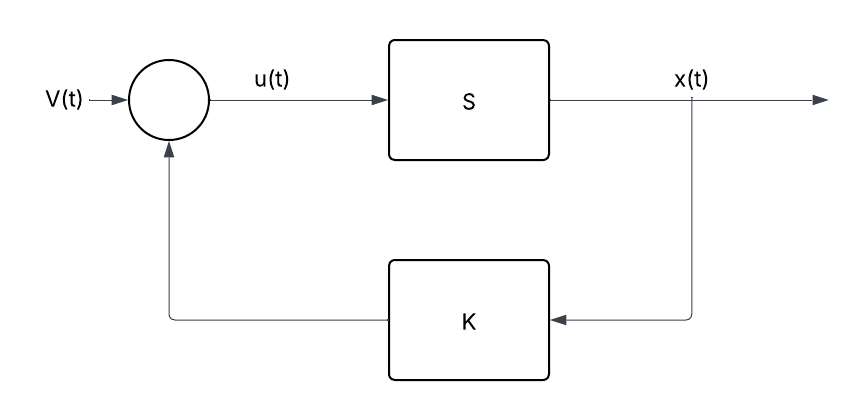
\includegraphics[width=0.5\textwidth]{foto/cph4/grafico.png}
          \end{center}
          Scegliendo a mio piacere i valori dei guadagni di K posso veramente
          imporre gli autovalori di $A - B K$ e quindi ottenere un sistema con
          le caratteristiche che voglio? Dipende da come sono fatti A e B; per
          rispondere in modo esaustivo a questa domanda occere introdurre lo
          studio di un'altra proprietà \textit{strutturale} dei sistemi LTI che
          si chiama proprietà di \textbf{controllabilità} o
          \textbf{raggiungibilità}, perché ci portano alla stessa conclusione
          nonostante siano proprietà diverse.

\end{itemize}
\section{Controllabilità e raggiungibilità}
Le due proprietà cercano di descrivere la possibilità di agire sul
comportamento del mio sistema andando a manipolare il segnale di ingresso
$u(t)$. Con \textit{raggiungibilità} si intende la possibilità di modificare lo
stato iniziale del sistema per raggiungere, appunto, uno stato desiderato. Con
\textit{controllabilità} si intende la possibilità di controllare a quale stato
finale arrivare partendo da uno stato iniziale, manipolando il segnale di
ingresso $u(t)$.
\subsection{Definizione formale di raggiungibilità}
Uno stato $x^*$ è raggiungibile se esistono:
\begin{itemize}
    \item un istante di tempo $t^* \in [t_0, \infty]$;
    \item un ingresso $u^*(t)$ definito per $t \in [t_0, \infty]$;
\end{itemize}
tali che la soluzione del sistema sia $x(t^*) = x^*$. L'insieme delle soluzioni
raggiungibili è chiamato insieme di raggiungibilità del sistema e costituisce un
sottospazio lineare dello spazio di stato X.
\begin{center}
    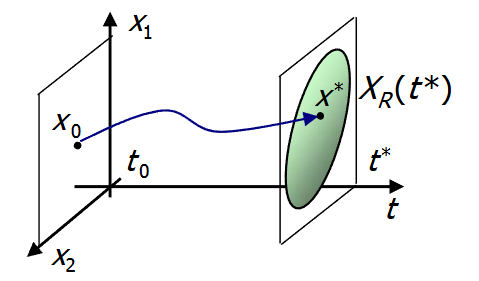
\includegraphics[width=0.5\textwidth]{foto/cph4/raggiungibilità.png}
\end{center}
{\bf Cosa succede se io estendo $t^*$ a $[t_0, \infty)$?} Quando $t^* \to
    \infty$, allora ho trovato tutti i punti di raggiungibilità e quindi
definisco l'insieme chiamato \textbf{sottospazio di raggiungibilità}. Quindi
$X_R = max(X_R(t))$; se $X_R = X$, allora dico che il sistema è
completamente raggiungibile, altrimenti dico che il sistema è parzialmente
raggiungibile. Il complemento ortogonale di $X_R$ è chiamato
\textbf{sottospazio di non raggiungibilità}.
\subsection{Definizione formale di controllabilità}
Uno stato $x^*$ è controllabile se esistono:
\begin{itemize}
    \item un istante di tempo $t^* \in [t_0, \infty)$;
    \item un ingresso $u^*(t)$ definito per $t \in [t_0, \infty)$;
\end{itemize}
tali che la soluzione del sistema sia $x(t^*) = x_0$. L'insieme delle soluzioni
controllabili è chiamato insieme di controllabilità del sistema e costituisce un
sottospazio lineare dello spazio di stato X.
\begin{center}
    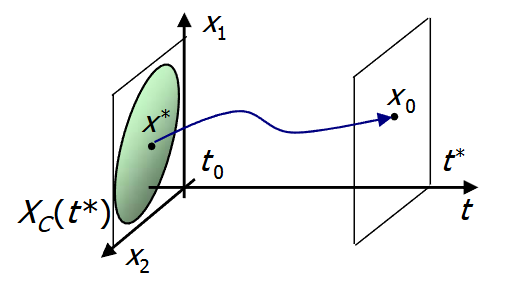
\includegraphics[width=0.5\textwidth]{foto/cph4/controllabilità.png}
\end{center}
\subsection{Considerazioni per sistemi LTI}
Per i sistemi LTI, la raggiungibilità e la controllabilità sono equivalenti,
quindi si ha che:
\begin{itemize}
    \item $X_R = X_C$
    \item $X_{NR} = X_{NC}$
    \item $X_R \subseteq  X_{NR} = X_C \subseteq X_{NC} = X$
    \item se la matrice A è non singolare, allora $X_R = X_C = X$
\end{itemize}
La controllabilità di un sistema dipende dalla sua struttura fisica,
\subsection{Come possiamo determinare $X_R$ per sistemi LTI TD}
Consideriamo un sistema LTI TD descritto dalle equazioni di stato:
\begin{equation}
    x(k+1) = A x(k) + B u(k)
\end{equation}
Vogliamo determinare:
\begin{itemize}
    \item l'insieme di raggiungibilità $X_R$ del sistema;
    \item il sottospazio di raggiungibilità $X_R$ del sistema;
    \item condizione necessaria e sufficiente affinché il sistema sia completamente
          raggiungibile.
\end{itemize}
Consideriamo il seguente caso:
\begin{tcolorbox}
    Supponiamo il sistema abbia un solo ingresso, ovvero $p=1 \rightarrow B \in
        \mathbb{R}^{n \times 1}$ e che la condizione iniziale sia nulla, ovvero
    $x(0) = 0$. Allora avremo che:
    \begin{align*}
        x(1) & = B u(0)                                                           \\
        x(2) & = A x(1) + B u(1) = A B u(0) + B u(1)                              \\
        x(3) & = A x(2) + B u(2) = A^2 B u(0) + A B u(1) + B u(2)                 \\
             & \vdots                                                             \\
        x(l) & = A^{l-1} B u(0) + A^{l-2} B u(1) + \cdots + A B u(l-2) + B u(l-1)
    \end{align*}
    con tempo discreto, quindi $l \in \mathbb{N}$ Si può compattare tutto come
    segue:
    \begin{equation}
        x(l) = [B, A B, A^2 B, \cdots, A^{l-1} B] \begin{bmatrix}
            u(l-1) \\
            u(l-2) \\
            \vdots \\
            u(0)
        \end{bmatrix} = M_r(l) U(l)
    \end{equation}
    La matrice $M_R(l) $ rappresenta il legame tra la sequenza in ingresso e lo
    stato del sistema al tempo $l$. Pertanto l'insisme di raggiungibilità
    $X_R(l)$ è dato da:
    \begin{equation}
        X_R(l) = \mathcal{R}(M_R(l)) = \mathcal{R} \{B, A B, A^2 B, \cdots, A^{l-1} B\}
    \end{equation}
    La grandezza del rango definisce la dimensione del sottospazio di
    raggiungibilità $X_R(l)$. So per certo che il numero di colonne che posso
    aggiungere è al massimo n, quindi se $l > n$, allora $X_R(l) = X_R(n)$. Lo
    spazio di raggiungibilità quindi è pari alla dimensione del sottospazio
    generato dalle colonne di $M_R(n)$. Un sistema dinamico LTI TD è
    completamente raggiungibile se e solo se il rango di $M_R(n)$ è pari a n.
\end{tcolorbox}

\section{Retroazione}
Per risolvere il problema di assegnazione degli autovalori, utilizziamo il
\textit{\textbf{Teorema di assegnazione degli autovalori}}, secondo cui se un
sistema è completamente raggiungibile, allora è possibile progettare una
matrice di guadagno K tale che gli autovalori di $A - B K$ siano quelli
desiderati.
\begin{tcolorbox}
    \begin{itemize}
        \item Voglio assegnare a $(A - B K)$ gli autovalori scelti da me che metto nel
              vettore $\lambda=[\lambda_1, \lambda_2, \cdots, \lambda_n]$;
        \item Verifico se il problema può essere risolto:
              \begin{verbatim}
                M_r = ctrb(A, B);
                r = rank(M_r);
                if r == n
                    disp('Il sistema è completamente raggiungibile');
                else
                    disp('Il sistema non è completamente raggiungibile');
                end
            \end{verbatim}
        \item Posso calcolare $k$ tale che \verb|eig(A-Bk)=\lambda| usando:
              \begin{verbatim}
                    k = place(A, B, lambda);
                    or 
                    k = acker(A, B, lambda);
            \end{verbatim}

    \end{itemize}
\end{tcolorbox}
\subsection{Il problema dell'assegnazione degli autovalori}
Vogliamo studiare sotto quali condizioni, tramite un'opportuna scelta della
matrice $K$, è possibile fare in modo che gli $n$ autovalori della matrice $(A
    - B K)$ coincidano con $n$ valori fissati. Una volta assegnati gli autovalori
desiderati, siamo in grado di progettare un sistema con le caratteristiche che
vogliamo. Le equazioni che descrivono il sistema retroazionato sono:
\begin{align*}
    \dot{x}(t) = Ax(t) + Bu(t) = A x(t) + B [-K x(t) + \alpha r(t)] = (A - B K) x(t) + B \alpha r(t) \\
    y(t) = C x(t) + D u(t) = C x(t) + D [-K x(t) + \alpha r(t)] = (C - D K) x(t) + D \alpha r(t)
\end{align*}
La matrice di trasferimento $H(s)$ del sistema retroazionato è data da:
\begin{equation}
    H(s) = \{ (C - D K) [sI - (A - B K)]^{-1} B + D \}\alpha
\end{equation}

\begin{tcolorbox}[title = Problema di regolazione]
    Tutto da prendere da file docente
    Ipotesi di lavoro:
    \begin{itemize}
        \item Possiamo misurare tutte le variabili di stato;
        \item il segnale di riferimento è del tipo $r(t) = R_0 \epsilon(t)$;
        \item rango di $M_r=n$ (completamente raggiungibile, altrimenti non posso risolvere
              il problema);
        \item \verb|k=place(A,B, lambda)|
    \end{itemize}
\end{tcolorbox}

\begin{tcolorbox}[title= Osservatore dello stato (stimatore assoluto dello stato)]
    Obiettivo: Costruire un dispositivo che utilizzando solo le informazioni disponibili ci fornisca una stima dello stato $\hat{x}(t)$ tal che $\hat{x}(t) \rightarrow x(t)$
    \begin{itemize}
        \item modello matematico del sistema(equazioni ingresso stato-uscita);
        \item $u(t), \forall t$;
        \item $y(t), \forall t$;
    \end{itemize}
    \begin{equation}
        S=
        \begin{cases}
            \dot{x}(t) = A x(t) + B u(t) \\
            y(t) = C x(t)
        \end{cases}
    \end{equation}
    \begin{equation}
        \sigma =
        \begin{cases}
            \dot{\hat{x}}(t) = A \hat{x}(t) + B u(t) - L (\hat{y(t)} - y(t)) \\
            \hat{y}(t) = C \hat{x}(t)
        \end{cases}
    \end{equation}
    Devo necessariamente inserire un termine di correzione $L (\hat{y(t)} - y(t))$ per fare in modo che la stima dello stato $\hat{x}(t)$ converga allo stato reale $x(t)$. $\hat{y}(t) = C \hat{x}(t)$ è la stima dell'uscita del sistema, mentre $y(t)=C x(t)$ è l'uscita reale del sistema.
    Il termine $(\hat{x(t)} - x(t))$ rappresenta l'errore di stima dello stato che chiameremo $e_x(t)$.
    Sostituendo nell'errore le equazioni di stato del sistema e dell'osservatore, ottengo:
    \begin{center}
        \begin{align*}
            e_x(t) = \hat{x}(t) - x(t)                                        \\
            \dot{e}_x(t) = \dot{\hat{x}}(t) - \dot{x}(t) =                    \\
            A \hat{x}(t) + B u(t) - L (\hat{y(t)} - y(t)) - A x(t) - B u(t) = \\
            (A - L C) e_x(t)
        \end{align*}
    \end{center}
    Osservazioni:
    \begin{itemize}
        \item l'errore di stima convergerà a zero se e solo se gli autovalori di $(A - L C)$
              sono tutti a parte reale negativa;
        \item inoltre il comportamento dell'errore di stima in transitorio dipende da come
              sono fatti gli autovalori di $(A - L C)$.
    \end{itemize}
\end{tcolorbox}
\section{Osservabilità}
L'osservabilità e la rilevabilità sono proprità che descrivono la possibilità
di stimare lo stato del sistema $x(\cdot)$ tramite la misura del movimento
dell'uscita $y(\cdot)$.
\begin{tcolorbox}[title= Definizione formale di osservabilità]
    La proprietà di osservabilità descrive la possibilità di stimare lo stato iniziale del sistema mediante la misura dell'uscita e dell'ingresso in un dato intervallo di tempo.
\end{tcolorbox}
\begin{tcolorbox}[title= Definizione formale di rilevabilità]
    La proprietà di rilevabilità descrive la possibilità di stimare lo stato finale del sistema mediante la misura dell'uscita e dell'ingresso in un dato intervallo di tempo.
\end{tcolorbox}
\hfill
\begin{minipage}{0.55\textwidth}
    Per poter studiare la proprietà di osservabilità è opportuno definire il
    concetto di non osservabilità. Uno stato $x^*$ si dice non osservabile se
    qualunque sia $t*$, il movimento libero dell'uscita conseguente allo stato
    iniziale $x^*$ è nullo. Quindi definiamo come sottospazio di osservabilità
    $X_O$ il complementare degli stati non osservabili del sistema. Gli stati
    osservabili possono influenzare la parte non osservabile, ma non viceversa.
\end{minipage}
\hfill
\begin{minipage}{0.4\textwidth}
    \centering
    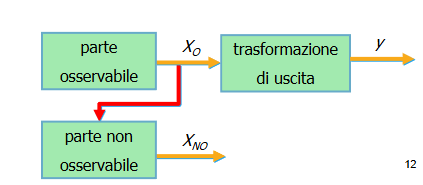
\includegraphics[width=0.9\textwidth]{foto/cph4/osservability.png}
\end{minipage}
\hfill
\begin{tcolorbox}
    Ipotizziamo per semplicità il caso in cui il sistema abbia una sola uscita e che l'ingresso sia nullo.
    Abbiamo che:
    \begin{align*}
        y(0) & = C x(0)              \\
        y(1) & = C x(1) = C A x(0)   \\
        y(2) & = C x(2) = C A^2 x(0) \\
             & \vdots                \\
        y(l) & = C x(l) = C A^l x(0)
    \end{align*}
    Possiamo compattare tutto come segue:
    \begin{equation}
        \begin{bmatrix}
            y(0)   \\
            y(1)   \\
            y(2)   \\
            \vdots \\
            y(l)
        \end{bmatrix} =
        \begin{bmatrix}
            C      \\
            C A    \\
            C A^2  \\
            \vdots \\
            C A^l
        \end{bmatrix} x(0) = M_O(l) x(0)
    \end{equation}
    La matrice $M_O(l)$ rappresenta il legame tra lo stato iniziale del sistema e la sequenza di uscite misurate. L'insieme di non osservabilità $X_{NO}(l)$ al tempo $l$  corrisponde allo spazio nullo della matrice $M_O(l)$.
    La matrice di osservabilità $M_O(l)$ ha al massimo n righe, quindi se $l > n$, allora $X_{NO}(l) = X_{NO}(n)$. La dimensione del sottospazio di non osservabilità $X_{NO}$ è minima quando il rango di $M_O(n)$ è massimo. Un sistema dinamico LTI TD è completamente osservabile se e solo se il rango di $M_O(n)$ è pari a n.
    \begin{tcolorbox}[title=Matlab]
        Per verificare se un sistema è completamente osservabile, è sufficiente calcolare il rango della matrice di osservabilità $M_O(n)$, che si ottiene utilizzando la funzione \verb|obsv| in MATLAB. Il codice per calcolare il rango è il seguente:
        \begin{verbatim}
    M_o = obsv(A, C);
    r = rank(M_o);
    \end{verbatim}
        Se $r == n$, allora il sistema è completamente osservabile, altrimenti il
        sistema non è completamente osservabile. Progettiamo la matrice di guadagno $L$
        dell'osservatore dello stato nel seguente modo:
        \begin{verbatim}
    L = place(A', C', lambda)';
    or
    L = acker(A', C', lambda)';
\end{verbatim}
        \verb|k = place(A,B,out)| calcola k tale che \verb|eig(A-Bk)=out|. Per imporre \verb|eig(A-LC)=out| osservo che $(A - L C) = (A' - C' L') \rightarrow L'$, quindi usare le trasposte
    \end{tcolorbox}
\end{tcolorbox}

